\section{実装}

わかるらんどのクライアントは
HTML/CSS/JavaScriptで実装されており、
通常のブラウザ上のWebアプリケーションとして動作する。
%
サーバは、
並列計算プリミティブである
\textit{Linda}\cite{Carriero:1989:LC:63334.63337}を
Webサーバ上に実装した
WebLinda\footnote{https://github.com/node-linda/linda}を用いて実装している。

\subsection{Linda}

Lindaは、
複数のプロセスで共有される空間を用いて
プロセス間通信やデータ共有をサポートする
分散並列処理を行うためのモデルである。
プロセスが共有する空間は\textbf{タプル空間} (Tuple Space) と呼ばれ、
タプル空間内のデータ (Tuple) を使って通信やデータ共有を行う (図\ref{linda})。
Lindaのモデルはきわめて単純であるが、
各クライアントやデバイス間で直接送信をする処理を記述する必要がなく,
柔軟で強力なプロセス間通信を容易に記述することができる。

\begin{figure}[h]
\centering
\fbox{
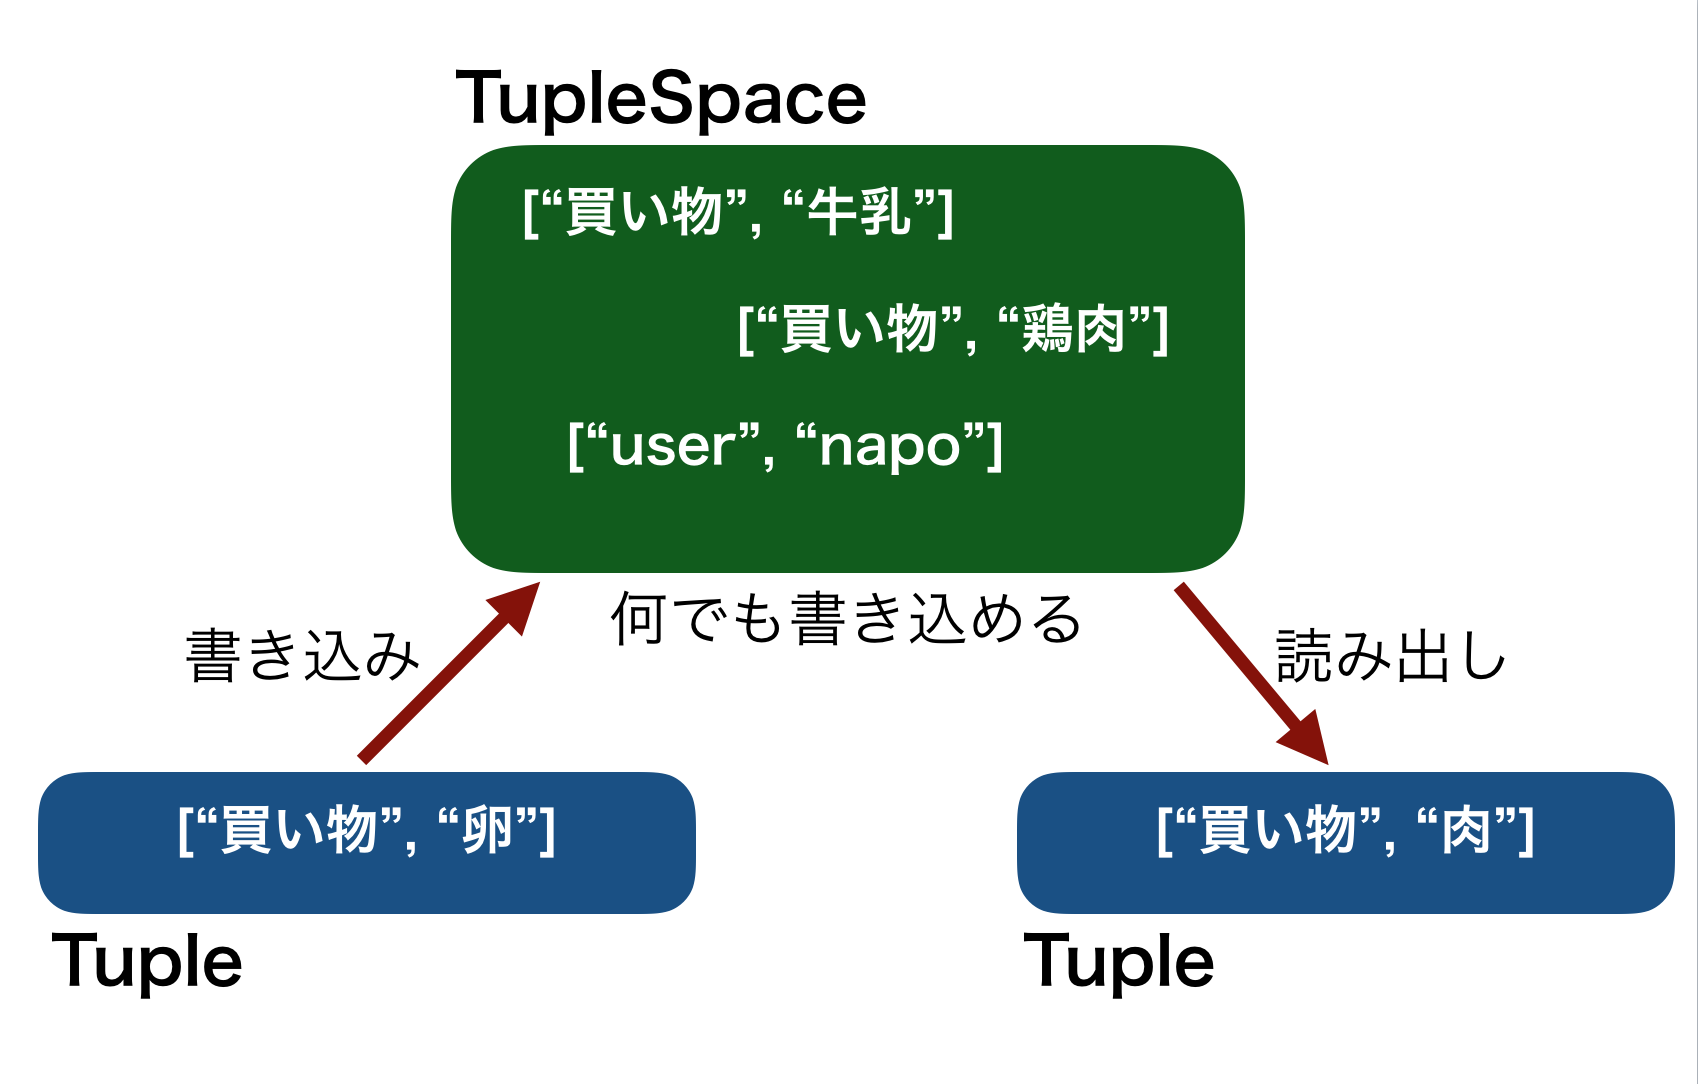
\includegraphics[width=7cm]{images/linda.png}
}
\caption{タプル空間を利用したプロセス間通信}
\label{button}
\end{figure}

\subsection{WebLinda}

WebLindaは、橋本翔氏が開発したオープンソースソフトウェアで、
% \footnote{http://shokai.org}
Node.js\footnote{https://nodejs.org}の
WebSocketライブラリ「Socket.IO\footnote{http://socket.io}」で
実装されている。
WebLindaは通常のWebサーバ上に実装されているため、
HTTP通信をサポートする様々な環境やプログラミング言語で利用可能である。

WebLindaは、\texttt{write}, \texttt{read}, \texttt{take}, \texttt{watch}という
4つの基本操作によってプロセス間通信を行う。

% ここは\enumerate じゃないのか?

\vspace{2mm}
\paragraph*{write}
新しいデータオブジェクト(タプル)を生成し共有空間(タプルスペース)に書き込む。

\vspace{4mm}
\paragraph*{read}
指定した形式に部分一致するタプルがタプルスペースにあるかどうか調べて1つ読み出す。
一致するものが無い場合は一致するタプルが書き込まれるまで待つ。

\vspace{2mm}
\paragraph*{take}
\texttt{read}しつつ、読み出したタプルをタプルスペースから削除する。

\vspace{2mm}
\paragraph*{watch}
タプルスペースを監視し、一致するタプルが\texttt{write}された瞬間に読み出す。

\subsection{『わかるらんど』でのWebLinda実装}
『わかるらんど』でのWebLinda実装について述べる。
ユーザのリアクションを投稿/表示する際には、
\begin{lstlisting}
{
    type: "reaction",
    from: "@napo0703",
    display: "60",
    value: "なる ほど"
}
\end{lstlisting}
というようなタプルをやりとりしている。

センサやWebのデータを投稿/表示する際には、
\begin{lstlisting}
{
    type: "data",
    from: "明るさ",
    display: "60",
    value: "500",
    background: "http://masuilab.org/image.jpg"
}
\end{lstlisting}
というようなタプルをやりとりしている。

\vspace{4mm}
\paragraph*{type}
ユーザのリアクションの場合は\texttt{reaction}、データの場合は\texttt{data}を値にする。

\vspace{4mm}
\paragraph*{from}
投稿元を表す値。

\vspace{2mm}
\paragraph*{display}
リアクションやデータの表示時間。単位は秒。リアクションやデータが表示されてからこの秒数が経過すると、自動的に取り下げられ表示されなくなる。20〜86400の間で指定が可能。

\vspace{2mm}
\paragraph*{value}
リアクションの場合、この値がWebにある画像ファイルのURLだった時は、その画像を投稿者のセルにオーバーレイ表示する。URLでない文字列の場合は、その文字列を投稿者のセルにオーバーレイ表示する。
データの場合、この値がそのままセルの下部に表示される。

\vspace{4mm}
\paragraph*{background}(データのみ)
データセルの背景画像のURL。そのデータが何を表すものなのか分かる画像を表示する。

\vspace{2mm}
以下は、ボタンを押した際に『わかるらんど』にユーザ「@napo0703」として「なる ほど」という「リアクション」を「20秒」表示するタプルを書き込むJavaScriptプログラムの例である。

\vspace{2mm}
\begin{lstlisting}
// Lindaに接続
const url = "http://linda.masuilab.org";
const socket = SocketIO(url);
const linda = new Linda().connect(socket);
const ts = linda.tuplespace("masuilab");

// ボタンを押したらタプルスペースにデータ書き込み
const button = $("button").click(function () {
  ts.write({
    type: "reaction",
    from: "@napo0703",
    display: "20",
    value: "http://masuilab.org/image.jpg",
  };
});
\end{lstlisting}

以下は、先程のプログラムで書き込まれるタプルと合致する
\texttt{{from: "@napo0703", type: "reaction"}}を含むタプルが書き込まれた場合に
リアクションを表示するJavaScriptプログラムの例である。

\vspace{2mm}
\begin{lstlisting}
// Lindaに接続
const url = "http://linda.masuilab.org";
const socket = SocketIO(url);
const linda = new Linda().connect(socket);
const ts = linda.tuplespace("masuilab");

// 合致するタプルが書き込まれたら画像を変える
ts.watch({
    from: "@napo0703",
    type: "reaction"
    }, function (tuple) {
  $("img").attr("src", tuple.data.value);
};
\end{lstlisting}

以下は現在の江ノ島の風向と風速をタプルスペースに書き込むRubyプログラムである。
NokogiriというライブラリでWebページから必要な情報をスクレイピングして
タプルスペースに書き込んでいる。

\vspace{2mm}
\begin{lstlisting}
url = 'http://linda.masuilab.org'
linda = Linda::SocketIO::Client.connect url
ts = linda.tuplespace('masuilab')

ts.on :connect do
  // Nokogiriでスクレイピング
  web = 'http://www.s-n-p.jp/kishou.htm'
  doc = Nokogiri::HTML(open(web))
  // 必要な情報を取得
  tds = doc.xpath("//td")
  as = tds[16].xpath(".//b").text.sub(/[^\d\.].*$/,'')
  ad = tds[19].xpath(“.//b”).text
  // タプルスペースに書き込み
  ts.write(
      where: 'enoshima',
      type: 'data',
      name: 'wind',
      value: ad + as.to_f + ‘m/s')
end
\end{lstlisting}